% $Author: stef $
% $Date: 2008-04-04 17:14:31 +0200 (Fri, 04 Apr 2008) $
% $Revision: 318 $
%=================================================================
\ifx\wholebook\relax\else
% --------------------------------------------
% Lulu:
    \documentclass[a4paper,10pt,twoside]{book}
    \usepackage[
        papersize={6in,9in},
        hmargin={.75in,.75in},
        vmargin={.75in,1in},
        ignoreheadfoot
    ]{geometry}
    \input{../common.tex}
    \pagestyle{headings}
    \setboolean{lulu}{true}
% --------------------------------------------
% A4:
%   \documentclass[a4paper,11pt,twoside]{book}
%   \input{../common.tex}
%   \usepackage{a4wide}
% --------------------------------------------
    \graphicspath{{figures/} {../figures/}}
    \begin{document}
%   \renewcommand{\nnbb}[2]{} % Disable editorial comments
    \sloppy
\fi

\chapter{Fun with Robots}\label{cha:fun}


\noindent\hrule
\begin{center}\includegraphics{beasts}\end{center}
\vspace{0.2cm}
\noindent\hrule\vspace{1.5cm}


The basic look of a robot is rather simple. Wouldn’t it be nice to be able to create robots that 
had a bit more pizzazz to them? Fortunately, you can create customized robots, and in this 
chapter, I will show you how you can change the shape, the pen size, and the color of your 
robots. You can make your robot look like an animal, a monster, or even the famous robot 
R2D2 from the movie Star Wars.


\section{Robot Handles}

You have learned about opening a message balloon for sending a message to a robot by click- 
ing on that robot. Now you are going to learn about obtaining access to other robot functions 
such as duplicating, moving, and changing the look of a robot. These extra functionalities are 
available via the halo of handles, which, as was mentioned briefly in Chapter 5, you can beam 
up by right clicking (command clicking on a Mac) on a robot. The handles are the small, 
round icons that surround the robot like a halo, as shown in Figure 6-1. I will explain the functions
 of the different handles as they are needed. You can get information about a handle by 
letting your mouse rest over a handle; then a balloon pops up and explains the handle’s 
purpose. For now, try to make a copy of the robot by clicking on the green (“duplicate the robot”) 
handle, move the robot by clicking on the black (“select the robot”) handle and dragging the 
robot, or destroy the robot using the pale pink (“destroy the robot”) handle with the “X.” 

\begin{figure}[h]
	\centerline{\includegraphics{picaAllHaloAnnotated}}
	\caption{Right click (command click) on the robot to bring up the halo of handles. \label{fig:halos}}
\end{figure}


\section{Pen Size and Color}

When our robots moved around the screen in previous chapters, they left a black trace in their 
wakes. But you are not limited to the default color black. You can change the color of a robot’s 
pen by sending a robot the message \ct{penColor:} with a color object as argument. One of the 
ways of obtaining a color object is to send a message with the name of a color to the class 
Color, which is a factory that makes color objects. For example, \ct{Color blue} yields a blue color 
object, and \ct{Color yellow} yields a yellow color object. Thus you can change the pen color of 
the robot \ct{pica} to the color blue with the message send \ct{pica penColor: Color blue}. I will 
explain more about colors in the following section. 

You can also change the thickness of the robot’s pen by sending the message penSize: 
with a number as argument. For example, \ct{pica penSize: 5} orders pica to change his pen size 
to be 5 pixels wide. Script~\ref{scr:pen} draws a thick blue line of width 5 pixels. 


\begin{script}[pen]{Pica can draw a thick blue line.}
| pica | 
pica := Bot new. 
!\textbf{pica penColor: Color blue.}!
pica go: 100. 
!\textbf{pica penSize: 5.}!
pica go: 100 
\end{script}





%%%%%%%%%%%%%%%%%%%%%%%%%%%%%%%%%%%%%%%%%%%%%%%%%%%%%%%%%%%%%%%%%%%%%%%%
\begin{scriptfigwithsize}[0.4]{
\includegraphics[width=5cm]{turtleMPenSize}}{Pica draws a spyglass.}\label{scr:spyglass}
| pica | 
pica := Bot new. 
pica go: 40. 
!\textbf{pica penSize: 2.}!
pica go: 40. 
!\textbf{pica penSize: 4.}!
pica go: 40. 
!\textbf{pica penSize: 6.}!
pica go: 40. 
\end{scriptfigwithsize}

You can change the color of the robot itself using the method \ct{color:}. For example, the 
message send \ct{berthe color: Color yellow} changes the robot \ct{berthe}’s color to yellow. Script~\ref{scr:color} tells \ct{berthe} to change her color to yellow and then go forward 100 pixels, while \ct{pica} is left 
behind with his default color and without moving.

\begin{script}[color]{Berthe changes her color and goes for a walk,while pica is left behind. }
	| pica berthe | 
	pica := Bot new. 
	berthe:= Bot new. 
	berthe color: Color yellow. 
	berthe go: 100. 
\end{script}

\section{More about Colors}

As previously mentioned, Squeak is an environment that is built from objects and that uses 
objects. Therefore, programming in Squeak amounts to creating objects and sending them 
messages. In particular, a color is an object created by the class \ct{Color}. 
To obtain a color object, you send a message to the class Color. 

Some color messages are named for the color they represent. For example, \ct{Color red} 
causes the class \ct{Color} to create a red color object. Here is the list of the predefined message 
selectors that you can send to the class \ct{Color} to create that color: \ct{black}, \ct{veryVeryDarkGray}, 
\ct{veryDarkGray}, \ct{darkGray}, \ct{gray}, \ct{lightGray}, \ct{veryLightGray},
\ct{veryVeryLightGray}~, \ct{white}, \ct{red}, \ct{yellow}, \ct{green}, \ct{cyan}, \ct{blue}, \ct{magenta}, \ct{brown}, \ct{orange}, \ct{lightRed}, \ct{lightYellow}, \ct{lightGreen}, \ct{lightCyan}, 
\ct{lightBlue}, \ct{lightMagenta}, \ct{lightBrown}, \ct{lightOrange}, \ct{paleBuff},
\ct{paleBlue}, \ct{paleYellow}, \ct{paleGreen}, \ct{paleRed}, \ct{veryPaleRed}, \ct{paleTan}, \ct{paleMagenta}, \ct{paleOrange}, and \ct{palePeach}. 

The \ct{Color} class is like a real-life paint factory. Not only can it make a large number of 
standard colors, it can also create a customized color for you by combining different amounts 
of red, green and blue. Table 6-1 shows a few examples of how to create colors this way using 
the message \ct{r:redAmount g: greenAmountb: blueAmount}. The arguments taken by the mes- 
sage selector \ct{r:g:b:} should be decimal numbers between 0 and 1 representing the amounts of 
red, green, and blue to be combined. For example, the expression \ct{Color r: 1 g: 0 b: 0} creates the same pure red color that you get from \ct{Color red}. Using the same amount of each of the three colors produces a shade of gray. All ones produces white, and all zeros produces  black. 

\noindent
\begin{table}[h!]
\caption{Creating Colors with \textsf{\upshape Color r:g:b:}}
\label{tab0601}
\begin{center}
{\small \begin{tabular}{p{20mm}p{20mm}p{20mm}p{20mm}}
\hline
{\small \textbf{Color}} & {\small \textbf{r: (Red)}} & {\small \textbf{g: (Green)}} & {\small \textbf{b: (Blue)}}\\
\hline
{\small red} & {\small 1} & {\small 0} & {\small 0}\\
{\small light gray} & {\small 0.1} & {\small 0.1} & {\small 0.1}\\
{\small yellow} & {\small 1} & {\small 1} & {\small 0}\\
{\small white} & {\small 1} & {\small 1} & {\small 1}\\
{\small black} & {\small 0} & {\small 0} & {\small 0}\\
{\small gray} & {\small 0.5} & {\small 0.5} & {\small 0.5}\\
{\small pale green} & {\small 0.8739} & {\small 1} & {\small 0.8348}\\
\hline
\end{tabular}}
\end{center}
\end{table}

Finally, the method \ct{fromUser} lets you pick a color from a palette on the screen, and then 
shows you that color’s ingredients, as illustrated in Figure~\ref{fig:palette} (though you will have to imagine 
the colors). For that, you need to execute the expression \ct{Color fromUser} using the print it 
menu to get the result of the selection printed. 

\begin{figure}[h]
	\centerline{\includegraphics{colorFromUser}}
	\caption{Choose your color from a color palette with the message send Color fromUser. 
	\label{fig:palette}}
\end{figure}

\section{Changing a Robot’s Shape and Size}

You can change a robot’s shape as well as its color. In addition to the default robot shape, two 
shapes, a circle and a triangle, are built into the \ct{Bot} factory (but you can also draw the robot 
shape with a drawing tool, as shown in the next section). The message \ct{lookLikeTriangle} gives 
a triangular shape to a robot. The message \ct{lookLikeCircle} gives a circular shape to a robot. 
The default shape is produced by sending the message \ct{lookLikeBot}. 

Another aspect you can change is the size of a robot using the message \ct{extent: widthAndHeight}, 
where the values of \ct{widthAndHeight} represent the width and height of the 
rectangle in which the robot is drawn. The argument \ct{widthAndHeight} is a pair of numbers, 
also called a point in Squeak. It is composed of two numbers separated by the \ct{@} symbol. 
For example, the point \ct{50@100} represents a rectangle 50 pixels wide and 100 pixels tall. 

Thus to create a robot named \ct{bigpica} in the shape of a triangle that fits inside a square 
with dimensions \ct{150@150}, you would first send \ct{bigpica} the message \ct{lookLikeTriangle} and 
then the message \ct{extent: 150@150}. 

Figure~\ref{fig:shapeAndSize} shows some robot shapes created using the built-in triangle and circle shapes, 
and Script~\ref{scr:shape} shows how to create robots of these sizes and shapes and move them into 
position as shown in the figure. 


\begin{figure}[h]
\begin{center}
\includegraphics[width=8cm]{shapeAndSize}
\caption{Robots can come in different shapes and sizes. \label{fig:shapeAndSize}}
\end{center}
\end{figure}


\begin{script}[shape]{Creating robots of different sizes and shapes (circles and triangles)}
| pica daly bigpica | 
pica := Bot new. 
pica lookLikeTriangle. 
pica west. 
pica color: Color red. 
pica penColor: Color green. 
pica penSize: 3. 
pica go: 100. 
daly := Bot new. 
daly extent: 60@60. 
daly east. 
daly go: 100. 
bigpica := Bot new. 
bigpica lookLikeTriangle. 
bigpica extent: 150@150. 
bigpica penSize: 5. 
bigpica north. 
bigpica go: 80. 
\end{script}

\section{Drawing Your Own Robot}

Squeak lets you draw a customized robot. You can even create a robot that looks like one of 
the figures shown at the beginning of this chapter. I will now describe step by step how to 
draw your own robot. 

\paragraph{Step 1:Open the painting tool via the red handle.}

The first step is to open the painting tool that is included in Squeak. Right click (or command click for Mac) to beam up the halo around the robot that you want to paint, as shown in Figure~\ref{fig:paintToolCaroFlap}. Click on the red 
handle, the one with the icon of a pen inside. This will open the painting editor, which 
is depicted in Figure~\ref{fig:paintOpen}. Do not worry about the other handles. Note that if you have 
already drawn a graphic, that graphic will be shown inside the painting tool. 


\begin{figure}[h]
\begin{center}
\includegraphics[width=6cm]{picaHaloAnnotated} 
\end{center}
\caption{Right click (or command click) to obtain the halo.Choose the painting editor 
from the red handle. \label{fig:paintToolCaroFlap}}
\end{figure}

\begin{figure}[h]
\begin{center}
\includegraphics[width=\textwidth]{paintOpen}
\caption{The painting editor. \label{fig:paintOpen}}
\end{center}
\end{figure}

\paragraph{Step 2: Draw the new robot graphic.}

The second step is to draw a new graphic for your robot. Draw your robot pointing to the right, as shown in Figure~\ref{fig:spottedspider}. The painting editor has the usual features of graphics programs, such as selecting the brush size, filling a 
region, repeating a selected region, and selecting the paint color. The painting tool also 
has two buttons (shown in Figure~\ref{fig:zoomandrotate}) to rotate and zoom your drawing. 


\begin{figure}[h]
\begin{center}
\includegraphics[width=\textwidth]{editingSpider}
\end{center}
\caption{This robot looks like a spotted spider.\label{fig:spottedspider}}
\end{figure}

\begin{figure}[h]
\begin{center}
\includegraphics[width=5cm]{zoomButton} \includegraphics[width=5cm]{rotateButton}
\end{center}
\caption{The zoom and rotate buttons. \label{fig:zoomandrotate}}
\end{figure}


\paragraph{Step 3:Preserving your graphic.}
Once you are satisfied with your drawing, you should 
press the button \button{keep}. This closes the painting tool. Now your robot looks like the graphic 
that you created. 

\section{Saving and Restoring Graphics}

If you have spent lot of time drawing a robot and you would like to save it for future reference, 
you can save it to a file. Once it has been saved, you will be able to load it into different 
environments and share it with your friends. You can begin to build a library of robot graphics over 
time. Now I will show you how to save and load a graphic. Then I will show how you can associate 
a graphic with a single robot or even to a class (robot factory), so that all newly created 
robots will look like the graphics that you have drawn. I will start by showing you how to 
perform all these manipulations by interacting with the robots directly, and then how to write 
scripts to do these things automatically.


\subsection{The “Save Graphics”Handle}

To save a graphic, simply click on the blue handle, the one with the file icon (Figure~\ref{fig:PicaHaloSaveAndLoadAnnotated}). 
I chose the color blue to make you think of a frozen lake: saving the graphic “freezes” your 
robot’s shape to preserve it. The system will then ask you to give a name to the saved graphic, 
as shown in Figure 6-9. This operation saves your graphic to a file, in the same folder as the 
Squeak image, with the name you entered and with the extension \ct{.frm}. 

\begin{figure}[h]
\begin{center}
\includegraphics{picaHaloSaveAndLoadAnnotated}
\end{center}
\caption{The robot now looks like a spider.It is pointing to the right.  \label{fig:PicaHaloSaveAndLoadAnnotated}}
\end{figure}

\begin{figure}[h]
\begin{center}
\includegraphics[width=\textwidth]{nameOfSaveAnnotated}
\end{center}
\caption{Clicking on the blue handle produces a prompt for a name.  \label{fig:prompt}}
\end{figure}

You can reverse the operation and load a graphic by clicking on the pink handle in the 
robot’s halo, the one with an icon that looks like a tool that a robot might use. I chose the color 
pink to make you think of bringing your robot back to life. When you click on the pink handle, 
the system asks you for the name of the graphic you want to load. Your robot will take on the 
appearance of the graphic that you choose.

\section{Retooling the Robot Factory}

You have drawn and saved a beautiful spotted spider, and you would like the robot factory 
to make you a robot with this graphic, but when you tell the \ct{Bot} class to create a new robot, 
it creates one using the default graphic. In order for the \ct{Bot} class to be able to create your 
spider robot, you have to tell your robot to pass its graphic to the class using the message 
\ct{passImageToClass}. After you have sent this message, if you create a new robot and ask it to 
look like the image, it will look like the graphic that you just drew. 

Another way of obtaining the same result is to send \ct{lookLikeImage} or any of the \ct{lookLike}
messages to the Bot class itself. Then the class will be configured to create new robots according to the new configuration. For example, if you send the message \ct{lookLikeCircle} to the 
class \ct{Bot}, all newly created robots will look like a circle. Thus if you want to have the Bot class 
create robots that look like spiders, you have to (1) get a robot, (2) draw the spider or load a 
previously saved spider graphic, (3) pass the spider image to the class, and (4) tell the class to 
make robots with the image by sending it the message \ct{lookLikeImage}. Then all your newly 
created robots will look like a spider, as shown in Figure~\ref{fig:allGraphics}.


\begin{figure}[h]
\begin{center}
\includegraphics[width=\textwidth]{allGraphics2}
\end{center}
\caption{Passing an image to the Bot class and sending the message lookLikeImageresults in 
all newly created robots looking like that image. \label{fig:allGraphics}}
\end{figure}

\section{Graphics Operations Using Scripts}

You can also write a script to load and save graphics and associate them with a single robot or 
with a class. 

Script~\ref{scr:load1} creates two robots and loads a graphic for each of them using two different 
methods. After picais created, he is sent the message \ct{loadImage}, which results in a prompt to 
the user for the name of the image to load. Then bertheis created, and she is sent the message 
\ct{loadImage: 'spider'}, which gives her the image contained in the image file \ct{spider.frm}. 

Note the important distinction between the messages \ct{loadImageandloadImage: 'fileName'}. 
The first of these has no parameter, and the user is prompted for the name of 
the graphics file to load. The second message does have a parameter, where here 'fileName' 
represents the name of the image file inside single quotation marks (and without the file 
extension). 

You can save the image using the message \ct{saveImage} or \ct{saveImage: 'fileName'}. First 
\ct{berthe} is sent the message \ct{saveImage}, which prompts the user for the name under which the 
image is to be saved. Finally, \ct{pica} is sent the message \ct{saveImage: 'spider2'}, which saves his 
image under the file name \ct{spider2.frm}. 




\begin{script}[load1]{Two ways of loading and saving robot graphics}
	| pica berthe | 
	pica := Bot new. 
	pica loadImage.             "The user is prompted for the name of the image to load" 
	berthe := Bot new. 
	berthe loadImage: 'spider'   "A parameter gives the name of the file to be loaded" 
	berthe saveImage.           "The user is prompted to name the saved image file" 
	pica saveImage: 'spider2'   "A parameter gives the name of the saved image" 
\end{script}

Just as you can load and save graphics associated with an individual robot, you can load 
and save graphics that are to be associated with a class, such as the Botclass. The same mes- 
sages are used for the class as were used for the individual robots. They are just sent to Bot 
instead of to \ct{pica}or \ct{berthe}. Script~\ref{scr:load2} first associates the image spider.frmwith the Botclass. 
Then the image is saved under another name, spiderBot.frm. 

Instead of the methods \ct{loadImage:} and \ct{saveImage:}, you can use \ct{loadImage} and \ct{saveImage} 
(no colon, no argument), which prompt the user for a file name. The expression \ct{Bot clearImage} 
resets the \ct{Bot} class to its condition the first time you used it. This restores the default robot 
image to the class, which means that when you run the script, you can reproduce a predictable 
scenario. 

\begin{script}[load2]{Loading and saving a graphic associated with the \ct{Bot} class}
| pica berthe | 
Bot clearImage.           "clears any graphic that was previously associated 
with the class Bot." 
berthe := Bot new.        "berthe looks like a default robot" 
Bot loadImage: 'spider'.  "The image in spider.frm is associated with the Bot class" 
Bot lookLikeImage 
pica := Bot new.          "The robot pica looks like a spider" 
Bot saveImage: 'spider3'  "The spider image is saved under the name spider3.frm" 
\end{script}




The following scripts (Script~\ref{scr:clear} and 6-8) assume that three image files, \ct{luth.frm}, 
\ct{spider.frm}, and \ct{airplane.frm} are located in the directory containing the Squeak image. 
These files are included in the distribution of the environment used in this book. 

Script~\ref{scr:clear} uses the method \ct{loadImage:} to associate an image with a robot, and the method 
\ct{lookLikeImage} to instruct a robot to look like the image with which it is associated. After the robot 
\ct{pica} is created, he is asked to look like his associated image (\ct{pica lookLikeImage}). Since no 
graphic has been associated with pica, asking him to look like an image produces no change. 
But then the image from the file \ct{luth.frm} is associated with \ct{pica} by sending him the message 
\ct{loadImage:'luth'}. Now when \ct{pica} is sent the message \ct{lookLikeImage}, his appearance is 
changed, and he looks like a luth sea turtle. In the last line of the script, a different image file is 
associated with pica. Once it has been given the message \ct{lookLikeImage}, a robot will look like 
whatever image is associated with it. Thus when the expression \ct{pica loadImage: 'spider'} is 
executed, \ct{pica} will look like a spider. 

The script continues with a new robot, \ct{berthe}, being created. Since the class \ct{Bot} does not 
have any image associated with it, \ct{berthe} will have the graphic of a default robot, and if you 
send her the message \ct{lookLikeImage}, nothing changes, since she does not have an associated 
image. 


\begin{script}[clear]{Changing the image of a robot}
	| pica berthe | 
	Bot clearImage. 
	pica := Bot new. 
	pica lookLikeImage. 
	"No image loaded or created, so nothing changes" 
	pica loadImage: 'luth'. 
	pica lookLikeImage 
	"Load an image and ask the robot to look like it" 
	pica loadImage: 'spider'. 
	"load another image, and since the message lookLikeImage has already been 
	sent, pica will look like the new image" 
	berthe := Bot new. 
	berthe lookLikeImage. 
	"When berthe is created, she looks like a default robot, and since no image 
	has been loaded into the class, the message lookLikeImage causes nothing to 
	change"
\end{script}

Script~\ref{scr:asso} shows how to notify the \ct{Bot} class that all newly created robots should have a 
particular graphic. In contrast to the situation described in Script~\ref{scr:clear}, the message \ct{loadImage: 'fileName'} is sent to the class \ct{Bot} itself and not to a particular robot. Just as a swimmer and a 
billiards player have different reactions to the word “pool,” different objects and classes have 
different understandings of the same message. That is because every object or class has its 
own method that responds to a given message, and these methods may be different for the 
same message. In the case at hand, \ct{loadImage:} has different behavior depending whether it is 
received by the \ct{Bot} class or by a robot, which is an instance of the class. When received by the
Bot class, the message \ct{loadImage: 'fileName'} leads to the class loading and associating the 
graphic from the file, so that newly created instances (robots) can use the new graphic. When 
received by a robot, only the particular robot receiving the message can use this graphic. 


\begin{script}[asso]{Associating a graphic with the \emph{Bot} class}
	| berthe daly pica yertle | 
	Bot loadImage: 'spider'. 
	berthe := Bot new. 
	berthe lookLikeImage. 
	"berthe, as an instance of the Bot class, now looks like a spider" 
	daly := Bot new. 
	daly lookLikeImage. 
	"daly also now looks like a spider" 
	pica := Bot new. 
	pica loadImage: 'luth'. 
	pica lookLikeImage. 
	"But a specific robot can still change its own graphics; 
	pica now looks like a turtle" 
	pica getImageFromClass. 
	"pica gets his image from the Bot class; now he looks like a spider again" 
	Bot loadImage: 'luth'. 
	Bot lookLikeImage. 
	yertle := Bot new. 
	"Now the class will create robots that look like luth turtles"
\end{script}

Script~\ref{scr:asso} starts by loading a new graphic from a file and associating it with the \ct{Bot} 
class  itself. Then the new robot \ct{berthe} is created, and she is sent the message that tells her to use 
the new graphic. Creating another robot, daly, and sending him the message \ct{lookLikeImage} 
makes him also look like the image associated with the class. 

All robots created can be made to look like a spider. However, a particular robot, such 
as the robot \ct{pica} in the script, can be given his own image by sending him the message 
\ct{loadImage: 'fileName'}. The robot’s associated image overrides the class image. The message 
\ct{getImageFromClass} makes it possible to restore the graphic associated with the class. The last 
sequence of messages shows that we can associate a new graphic to a class, replacing the 
currently associated image. Sending the message \ct{loadImage: 'fileName'} to the class \ct{Bot} 
associates the graphic in the file \ct{fileName.frm} to the class. Then sending the message 
\ct{lookLikeImage} ensures that newly created robots will by default look like the graphic 
now associated with the class. Hence the robot \ct{yertle} looks like a turtle. 


\section{Summary}
\noindent
{\small \begin{tabular}{p{20mm}p{50mm}p{30mm}}
\hline
\textbf{Method} & \textbf{Description} & \textbf{Example}\\
\hline
\textsf{lookLikeCircle} & Change the shape of the receiver to a circle. & \textsf{Bot new lookLikeCircle} \\

\textsf{lookLikeBot} & Change the shape of the receiver to a robot. & \textsf{Bot new lookLikeBot} \\

\textsf{lookLikeTriangle} & Change the shape of the receiver to a triangle. & \textsf{Bot new lookLikeTriangle} \\

\textsf{lookLikeImage} & Change the appearance of the receiver to the graphic you painted. & \textsf{Bot new lookLikeImage} \\

\textsf{lookLikeCircle} & Sending to the class results in newly created robots having the shape of a circle. 
& \textsf{Bot lookLikeCircle} \\

\textsf{lookLikeBot} & Sending to the class results in newly created robots having the shape of a robot. & \textsf{Bot lookLikeBot} \\

\textsf{lookLikeTriangle} & Sending to the class results in newly created robots having the shape of a triangle. 
& \textsf{Bot lookLikeTriangle} \\

\textsf{lookLikeImage} & Sending to the class results in newly created robots having the shape of the graphic you painted or loaded. & \textsf{Bot lookLikeImage} \\

\textsf{loadImage: '{\itshape fileName}'} & Load the image file \emph{fileName.frm} into the class or the robot.
& \textsf{Bot loadImage: 'spider'} \newline or \newline \textsf{berthe loadImage: 'spider'} \\

\textsf{loadImage} & Prompt the user for the name of an image file to be loaded into the class or the robot. 
& \textsf{Bot loadImage} or \newline  \textsf{berthe loadImage} \\

\textsf{saveImage: '{\itshape fileName}'} & Save the image of the class or the robot to the file named 
\emph{fileName.frm}. & \textsf{Bot saveImage: 'spider'} \newline or \newline  \textsf{berthe saveImage: 'spider'} \\

\textsf{saveImage} & Save the image of the class or the robot by prompting the user for a file name. 
& \textsf{Bot saveImage} or \newline  \textsf{berthe saveImage} \\

\textsf{penColor: {\itshape aColor}} & 
Change the color of the pen.
& \textsf{berthe penColor: Color blue} \\
\hline
\end{tabular}}

\noindent
{\small \begin{tabular}{p{20mm}p{50mm}p{30mm}}
\hline
\textbf{Method} & \textbf{Description} & \textbf{Example}\\
\hline

\textsf{penSize: {\itshape aNumber}} & 
Change the size of the pen. The default size is 1. 
& \textsf{berthe penSize: 3} \\

\textsf{color: {\itshape aColor}} & Change the color of the receiver to the specified color. 
& \textsf{berthe color: Color yellow} \\ 

\textsf{extent: {\itshape aPoint}} & Change the size of the receiver to dimensions given by \textsf{aPoint}
where \textsf{aPoint} is given by \textsf{w@h}, where \textsf{w} is the width and \textsf{h} is the height. & \textsf{berthe extent: 80@100} \\

 \textsf{passImageToClass} & Pass the graphic of the receiver to the class. After this message, robots created by the class will have as graphic the graphic of the current robot. & \textsf{berthe passImageToClass} \\
 
 \textsf{getImageFromClass} & Get the graphic of the class. After this message, the receiver will look like the robots that would be created by the class.  & \textsf{berthe getImageFromClass} \\
\hline
\end{tabular}}


%% %%%%%%%%%%%%%%%%%%%%%%%%%%%%%%%%%%%%%%%%%%%%%%%%%%%%%%%%%%%%%%%%%%%%%%%
% \begin{exofigwithsize}[0.5]{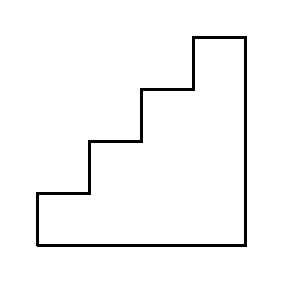
\includegraphics[width=3cm]{turtleMSmallStairs}}{A Staircase}\label{xp:letterA}
% You are not limited in your robot drawings to squares. You can create a wide range of geometrical figures.
% For example, here is a drawing of a small staircase. Write a script to reproduce this drawing. 
% \end{exofigwithsize}
% %%%%%%%%%%%%%%%%%%%%%%%%%%%%%%%%%%%%%%%%%%%%%%%%%%%%%%%%%%%%%%%%%%%%%%%%
% \begin{exonofigtitle}{Moving Clock Hands}
% Experiment with different angle values for each of the two robots; that is,change the angle values for the two turn 
% methods. Then, compare the effect of the method \ct{turnLeft: 60} (for pica) and \ct{turnRight: 300} (for daly). 
% You can see that turning left 60 degrees yields the same result as turning right 300 degrees. This is so because 
% the sum of the two values is 360 degrees, that is, a full circle. 
% \end{exonofigtitle}

\ifx\wholebook\relax\else
    \end{document}
\fi

%%% Local Variables:
%%% coding: utf-8
%%% mode: latex
%%% TeX-master: t
%%% TeX-PDF-mode: t
%%% ispell-local-dictionary: "english"
%%% End:
